\documentclass[10pt, a4paper]{article}

\usepackage{ctex}
\usepackage{xeCJK}
\usepackage{caption}
\usepackage{geometry}
\geometry{
    left = 0.6in,
    right = 0.6in,
    top = 0.8in,
    bottom = 1.0in
}
\usepackage{amssymb}
\usepackage{amsbsy}
\usepackage{amsmath}
\usepackage{xcolor}
\usepackage{mathrsfs}
\usepackage{graphicx}
\usepackage{pifont}
\usepackage{tikz}
\usepackage{tasks}
\settasks{
    label = \Alph*. ,
    label-width = 16pt
}

\newcommand{\Title}[3]{
    \begin{center}
        \Large \textbf{中国电子学会 #1~年~#2~月 Scratch~#3级考试}
    \end{center}
}
\newcommand{\TimeAndName}[1]{
    \begin{center}
        考试时间:~#1~ 分钟 \qquad\qquad\qquad\qquad 姓名:\underline{\quad\quad\quad\quad}
    \end{center}
}
\pagestyle{empty}
\begin{document}
    \Title{2020}{6}{一}
    
    \TimeAndName{60}
    
    {\noindent\heiti 第一部分、单选题(共 25 题,每题 2 分,共50分.)}

    \begin{enumerate}
        % 1
        \item 以下哪段程序可以实现小猫向左移动?(\qquad)
        \begin{tasks}(4)
            \task 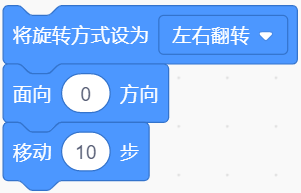
\includegraphics[width=.15\textwidth]{1a.png}
            \task 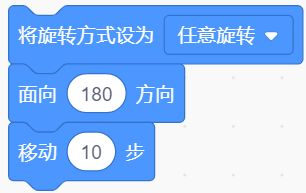
\includegraphics[width=.15\textwidth]{1b.png}
            \task 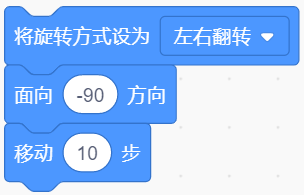
\includegraphics[width=.15\textwidth]{1c.png}
            \task 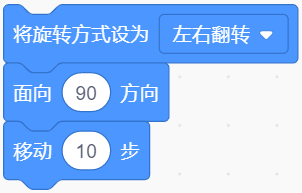
\includegraphics[width=.15\textwidth]{1d.png}
        \end{tasks}

        % 2
        \item 小猫给公园设计了如下的平面图,它想把黑色的路变成棕色,请问需要点击几次油漆桶按钮?(\qquad)
        \begin{tasks}(4)
            \task 3
            \task 9
            \task 1
            \task 10
        \end{tasks}

        % 3
        \item 默认的小猫有两个造型(分别为造型1和造型2)。在运行下面的程序后,没有看到造型的切换,下面哪一项可以修复这个问题?(\qquad)
        \begin{tasks}(2)
            \task 修改为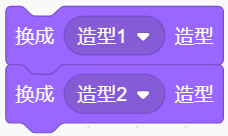
\includegraphics[width=.12\textwidth]{3a.png}
            \task 修改为
\includegraphics[width=.08\textwidth]{3b.png}
            \task 编辑小猫的造型
            \task 删除小猫的第一个造型:造型1
        \end{tasks}

        \begin{figure}[htbp]
            \centering
            \begin{minipage}[t]{.2\textwidth}
                \centering
                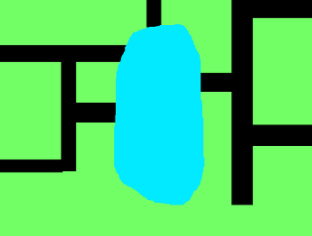
\includegraphics[width=1\textwidth]{2.png}
                \caption*{第2题}
            \end{minipage}
            \begin{minipage}[t]{.14\textwidth}
                \centering
                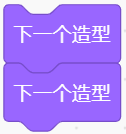
\includegraphics[width=\textwidth]{3.png}
                \caption*{第3题}
            \end{minipage}
            \begin{minipage}[t]{.22\textwidth}
                \centering
                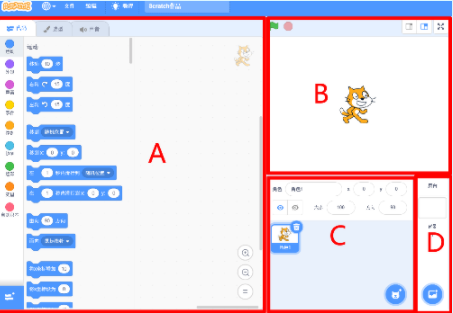
\includegraphics[width=\textwidth]{4.png}
                \caption*{第4题}
            \end{minipage}
            \begin{minipage}[t]{.22\textwidth}
                \centering
                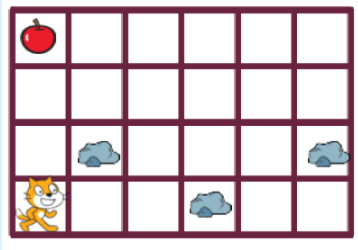
\includegraphics[width=\textwidth]{5.png}
                \caption*{第5题}
            \end{minipage}
        \end{figure}

        % 4
        \item 上面哪个区域是“舞台”?(\qquad)
        \begin{tasks}(4)
            \task A
            \task B
            \task C
            \task D
        \end{tasks}

        % 5
        \item 上面地图中每格的长度是50步长,小猫要想拿到苹果,下面哪组程序可以实现?(\qquad)
        \begin{tasks}(4)
            \task 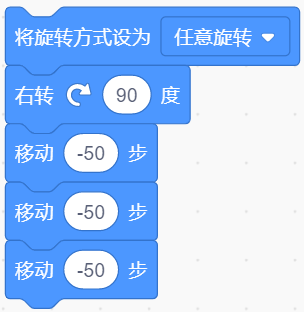
\includegraphics[width=.15\textwidth]{5a.png}
            \task 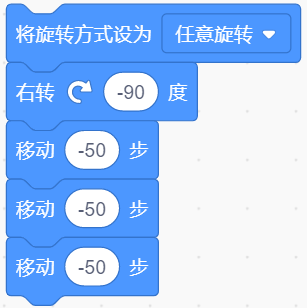
\includegraphics[width=.15\textwidth]{5b.png}
            \task 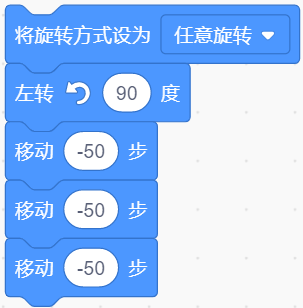
\includegraphics[width=.15\textwidth]{5c.png}
            \task 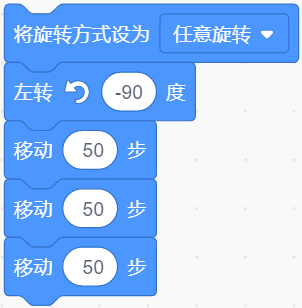
\includegraphics[width=.15\textwidth]{5d.png}
        \end{tasks}

        % 6
        \item 以下哪个可以实现小猫向上移动?(\qquad)
        \begin{tasks}(4)
            \task 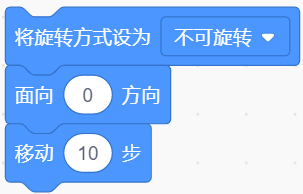
\includegraphics[width=.15\textwidth]{6a.png}
            \task 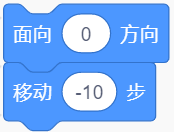
\includegraphics[width=.13\textwidth]{6b.png}
            \task 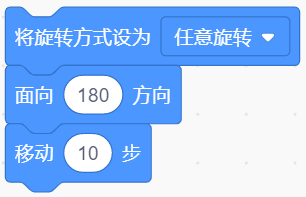
\includegraphics[width=.15\textwidth]{6c.png}
            \task 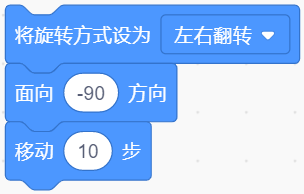
\includegraphics[width=.15\textwidth]{6d.png}
        \end{tasks}

        % 7
        \item 下面地图中每格的长度是50步长,小猫要想拿到苹果,下面哪组程序可以实现?(\qquad)
        \begin{tasks}(4)
            \task 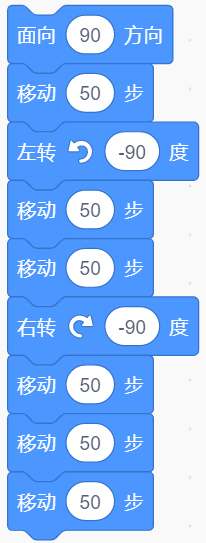
\includegraphics[width=.12\textwidth]{7a.png}
            \task 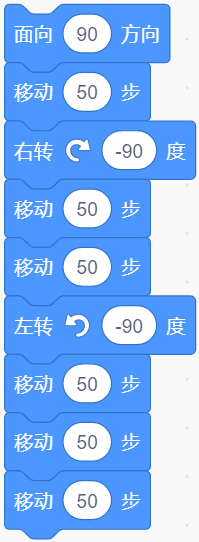
\includegraphics[width=.12\textwidth]{7b.png}
            \task 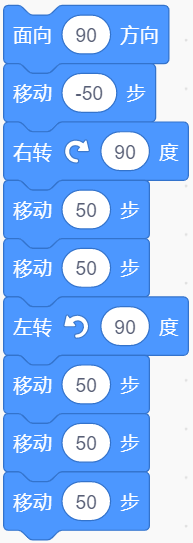
\includegraphics[width=.12\textwidth]{7c.png}
            \task 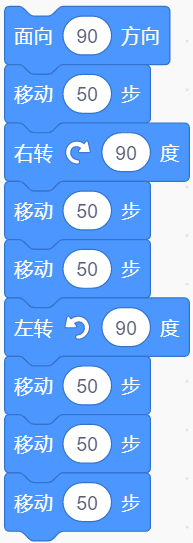
\includegraphics[width=.12\textwidth]{7d.png}
        \end{tasks}
           
        \item 以下哪个按钮可以实现造型水平翻转功能?(\qquad)
        \begin{tasks}(4)
            \task 
\includegraphics[width=.03\textwidth]{8a.png}
            \task 
\includegraphics[width=.03\textwidth]{8b.png}
            \task 
\includegraphics[width=.03\textwidth]{8c.png}
            \task 
\includegraphics[width=.02\textwidth]{8d.png}
        \end{tasks}

        \begin{figure}[htbp]
            \centering
            \begin{minipage}[t]{.2\textwidth}
                \centering
                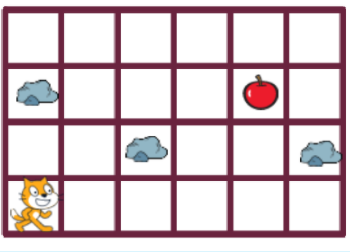
\includegraphics[width=\textwidth]{7.png}
                \caption*{第7题}
            \end{minipage}
            \begin{minipage}[t]{.21\textwidth}
                \centering
                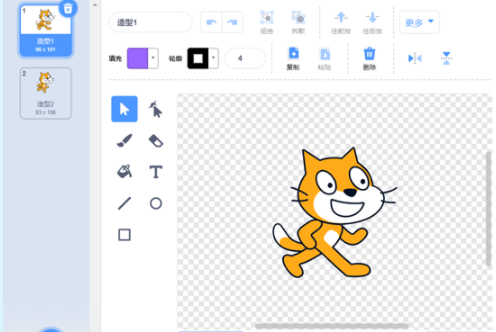
\includegraphics[width=\textwidth]{8.png}
                \caption*{第8题}
            \end{minipage}
            \begin{minipage}[t]{.2\textwidth}
                \centering
                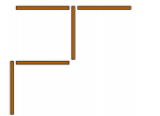
\includegraphics[width=\textwidth]{9.png}
                \caption*{第9题}
            \end{minipage}
            \begin{minipage}[t]{.14\textwidth}
                \centering
                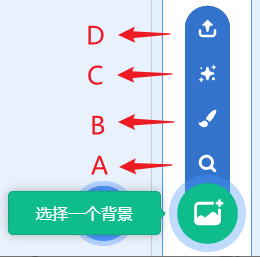
\includegraphics[width=\textwidth]{11.png}
                \caption*{第11题}
            \end{minipage}
            \begin{minipage}[t]{.21\textwidth}
                \centering
                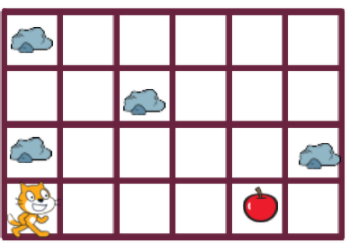
\includegraphics[width=\textwidth]{12.png}
                \caption*{第12题}
            \end{minipage}
        \end{figure}

        % 9
        \item 在上面图形基础上,只能移动一根火柴棍,不能变成下面哪个选项的图形?(\qquad)
        \begin{tasks}(4)
            \task 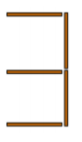
\includegraphics[width=.04\textwidth]{9a.png}
            \task 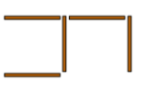
\includegraphics[width=.12\textwidth]{9b.png}
            \task 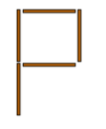
\includegraphics[width=.06\textwidth]{9c.png}
            \task 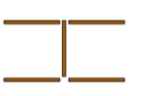
\includegraphics[width=.12\textwidth]{9d.png}
        \end{tasks}

        % 10
        \item 以下哪组积木块可以实现播放4次声音“喵”?(\qquad)
        \begin{tasks}(4)
            \task 
\includegraphics[width=.15\textwidth]{10a.png}
            \task 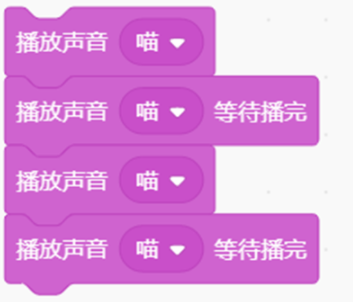
\includegraphics[width=.16\textwidth]{10b.png}
            \task 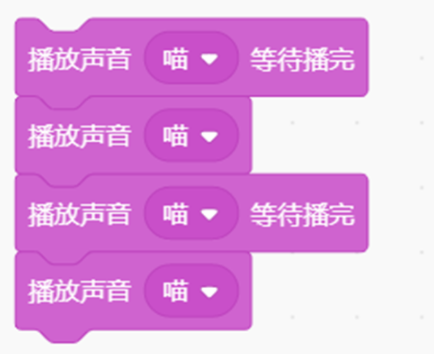
\includegraphics[width=.17\textwidth]{10c.png}
            \task 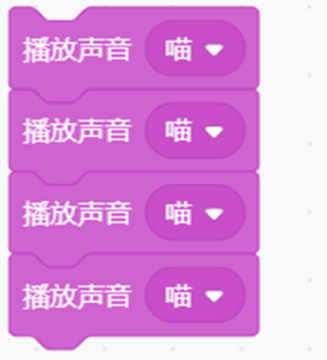
\includegraphics[width=.125\textwidth]{10d.png}
        \end{tasks}

        % 11
        \item 如上图,从背景库中选择一个背景,应该点击哪一个按钮?(\qquad)
        \begin{tasks}(4)
            \task A
            \task B
            \task C
            \task D
        \end{tasks}
        
        % 12
        \item 如上图,地图中每格的长度是50步长,小猫要想拿到苹果,下面哪组程序可以实现?(\qquad)
        \begin{tasks}(4)
            \task 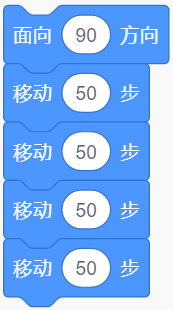
\includegraphics[width=.1\textwidth]{12a.png}
            \task 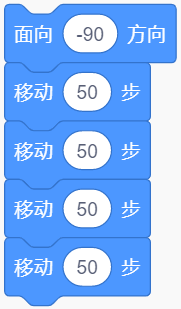
\includegraphics[width=.1\textwidth]{12b.png}
            \task 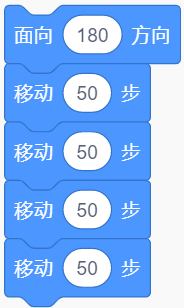
\includegraphics[width=.1\textwidth]{12c.png}
            \task 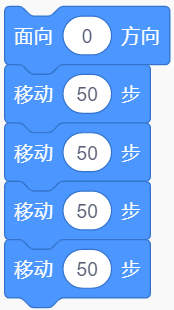
\includegraphics[width=.1\textwidth]{12d.png}
        \end{tasks}

        % 13
        \item 在菜单栏中以下哪个可以实现语言的切换?(\qquad)
        \begin{tasks}(4)
            \task 
\includegraphics[width=.05\textwidth]{13a.png}
            \task 
\includegraphics[width=.05\textwidth]{13b.png}
            \task 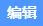
\includegraphics[width=.05\textwidth]{13c.png}
            \task 
\includegraphics[width=.07\textwidth]{13d.png}
        \end{tasks}

        % 14
        \item 下图为造型的编辑界面,以下哪个可以实现变形功能?(\qquad)
        \begin{tasks}(4)
            \task 
\includegraphics[width=.03\textwidth]{14a.png}
            \task 
\includegraphics[width=.03\textwidth]{14b.png}
            \task 
\includegraphics[width=.03\textwidth]{14c.png}
            \task \includegraphics[width=.03\textwidth]{14d.png}
        \end{tasks}
    
        % 15
        \item 如下图,想要录制一个声音,应该点击哪个按钮?(\qquad)
        \begin{tasks}(4)
            \task A
            \task B
            \task C
            \task D
        \end{tasks}

        \begin{figure}[htbp]
            \centering
            \begin{minipage}[t]{.2\textwidth}
                \centering
                \includegraphics[width=\textwidth]{14.png}
                \caption*{第14题}
            \end{minipage}
            \begin{minipage}[t]{.2\textwidth}
                \centering
                \includegraphics[width=\textwidth]{15.png}
                \caption*{第15题}
            \end{minipage}
            \begin{minipage}[t]{.23\textwidth}
                \centering
                \includegraphics[width=\textwidth]{16.png}
                \caption*{第16题}
            \end{minipage}
            \begin{minipage}[t]{.2\textwidth}
                \centering
                \includegraphics[width=\textwidth]{18.png}
                \caption*{第18题}
            \end{minipage}
        \end{figure}
        
        % 16
        \item 如上图,哪组积木块可以实现如下图小猫面向下移动?(\qquad)
        \begin{tasks}(4)
            \task \includegraphics[width=.1\textwidth]{16a.png}
            \task \includegraphics[width=.1\textwidth]{16b.png}
            \task \includegraphics[width=.1\textwidth]{16c.png}
            \task \includegraphics[width=.1\textwidth]{16d.png}
        \end{tasks}

        % 17
        \item 在声音编辑器中,能够实现声音头和尾互换,应该选择以下哪一个?(\qquad)
        \begin{tasks}(4)
            \task \includegraphics[width=.05\textwidth]{17a.png}
            \task \includegraphics[width=.05\textwidth]{17b.png}
            \task \includegraphics[width=.04\textwidth]{17c.png}
            \task \includegraphics[width=.05\textwidth]{17d.png}
        \end{tasks}

        % 18
        \item 上图为造型编辑界面,以下哪个可以实现造型垂直翻转功能?(\qquad)
        \begin{tasks}(4)
            \task \includegraphics[width=.05\textwidth]{18a.png}
            \task \includegraphics[width=.05\textwidth]{18b.png}
            \task \includegraphics[width=.04\textwidth]{18c.png}
            \task \includegraphics[width=.05\textwidth]{18d.png}
        \end{tasks}

        % 19
        \item 下面哪个区域是角色列表区?(\qquad)
        \begin{tasks}(4)
            \task A
            \task B
            \task C
            \task D
        \end{tasks}

        % 20
        \item 如下图,小猫去学校一共有几条路径?(\qquad)
        \begin{tasks}(4)
            \task 1
            \task 2
            \task 3
            \task 4
        \end{tasks}

        \begin{figure}[htbp]
            \centering
            \begin{minipage}[t]{.15\textwidth}
                \centering
                \includegraphics[width=\textwidth]{19.png}
                \caption*{第19题}
            \end{minipage}
            \begin{minipage}[t]{.23\textwidth}
                \centering
                \includegraphics[width=\textwidth]{20.png}
                \caption*{第20题}
            \end{minipage}
            \begin{minipage}[t]{.27\textwidth}
                \centering
                \includegraphics[width=\textwidth]{21.png}
                \caption*{第21题}
            \end{minipage}
        \end{figure}

        % 21
        \item 如上图,以下哪组积木块可以实现如下图小猫面向上移动?(\qquad)
        \begin{tasks}(4)
            \task \includegraphics[width=.1\textwidth]{21a.png}
            \task \includegraphics[width=.1\textwidth]{21b.png}
            \task \includegraphics[width=.1\textwidth]{21c.png}
            \task \includegraphics[width=.1\textwidth]{21d.png}
        \end{tasks}

        \newpage
        % 22
        \item 关于造型的说法正确的是?(\qquad)
        \begin{tasks}(2)
            \task 角色中有且只有一个造型
            \task 角色中必须有多个造型
            \task 角色中至少有一个造型
            \task 角色中可以没有造型
        \end{tasks}

        % 23
        \item 舞台背景与角色相比,哪个模块是没有的?(\qquad)
        \begin{tasks}(4)
            \task 运动模块
            \task 外观模块
            \task 声音模块
            \task 事件模块
        \end{tasks}

        % 24
        \item 找规律填数17,12,15,14,13,(\quad),(\quad)?(\qquad)
        \begin{tasks}(4)
            \task 16,11
            \task 12,11
            \task 14,15
            \task 12,7
        \end{tasks}
        
        % 25
        \item 如果将声音的音量设定为最大,那么音量的最大值是?(\qquad)
        \begin{tasks}(4)
            \task 240
            \task 180
            \task 255
            \task 100
        \end{tasks}
    \end{enumerate}

    % \begin{figure}[htbp]
    %     \centering
    %     \begin{minipage}[t]{.23\textwidth}
    %         \centering
    %         \includegraphics[width=\textwidth]{25.png}
    %         \caption*{第25题}
    %     \end{minipage}
    %     \begin{minipage}[t]{.23\textwidth}
    %         \centering
    %         \begin{minipage}[t]{.23\textwidth}
    %             \centering
    %             \includegraphics[width=\textwidth]{28-1.png}
    %         \end{minipage}
    %         \begin{minipage}[t]{.7\textwidth}
    %             \centering
    %             \includegraphics[width=\textwidth]{28-2.png}
    %         \end{minipage}
    %         \caption*{第28题}
    %     \end{minipage}
    %     \begin{minipage}[t]{.23\textwidth}
    %         \centering
    %         \includegraphics[width=\textwidth]{30.png}
    %         \caption*{第30题}
    %     \end{minipage}
    %     \begin{minipage}[t]{.13\textwidth}
    %         \centering
    %         \includegraphics[width=\textwidth]{33.png}
    %         \caption*{第33题}
    %     \end{minipage}
    % \end{figure}

    {\noindent\heiti 第二部分、判断题(共 10 题,每题 2 分,共20分.)}
    \begin{enumerate}
        \setcounter{enumi}{25}
        % 26
        \item 如图\includegraphics[width=.1\textwidth]{26.png}所示积木可以实现角色的位置移动.(\qquad)

        %27
        \item 添加舞台背景可以在角色列表区找到相应的选项.(\qquad)
        
        %28
        \item 执行\includegraphics[width=.15\textwidth]{28.png}程序,小猫一边叫一声“喵”一边向前走50步.(\qquad)
  
        %29
        \item 要获取当前音量大小值可以用\includegraphics[width=.12\textwidth]{29.png}积木.(\qquad)
        
        %30
        \item 在角色列表区的任意空白区域点击鼠标右键,会弹出一个菜单,可以对角色进行“复制”、“导出”、“删除”的操作.(\qquad)

        %31
        \item 如图所示积木\includegraphics[width=.12\textwidth]{31.png}的运算结果是35.(\qquad)
        
        %32
        \item 绘制背景可以选择\includegraphics[width=.02\textwidth]{32.png}按钮.(\qquad)
        
        %33
        \item 要实现音量的减小可以用\includegraphics[width=.12\textwidth]{33.png}积木.(\qquad)
        
        %34
        \item 要实现角色切换到指定的造型可以用\includegraphics[width=.08\textwidth]{34.png}积木.(\qquad)
        
        %35
        \item 用\includegraphics[width=.12\textwidth]{35.png}积木可以实现角色瞬间移动到指定坐标位置.(\qquad)
    \end{enumerate}

    \newpage
    {\noindent\heiti 第三部分、编程题(共 2 题,共30分.)}
    \begin{enumerate}
        \setcounter{enumi}{35}
        
        %36
        \item 球飞了:
        \begin{figure}[htbp]
            \begin{minipage}{.6\textwidth}
                1. 准备工作
                \begin{tasks}[label = (\arabic*)]
                    \task 背景:Pool;
                    \task 角色:Cat Flying、Ball.
                \end{tasks}
                2. 功能实现
                \begin{tasks}[label = (\arabic*)]
                    \task 分别添加角色Cat Flying、Ball和背景Pool;
                    \task 程序开始,Cat Flying向球游去,边游边切换造型,到达球的位置;
                    \task 小猫到达球的位置后,点击球,Ball向上飞;
                    \task Cat Flying说:“哎,球飞了”。
                \end{tasks}
            \end{minipage}
            \begin{minipage}{.37\textwidth}
                \centering
                \includegraphics[width=\textwidth]{36.png}
            \end{minipage}
        \end{figure}
            
        % 37
        \item 希神吓走猫头鹰:
        
        \begin{figure}[htbp]
            \begin{minipage}{.6\textwidth}
                1. 准备工作
                \begin{tasks}[label = (\arabic*)]
                    \task 背景:Forest;
                    \task 角色:Centaur,Owl.
                \end{tasks}
                2. 功能实现
                \begin{tasks}[label = (\arabic*)]
                    \task 分别添加角色Centaur,Owl和背景Forest;
                    \task 程序开始,角色OWI在舞台右上方,与Centaur面对面;
                    示;
                    \task 程序开始,Centaur切换为造型centaur-a,1秒后切换为造型centaur-d,并播放声音Meow2,然后切换为造型centaur-a;
                    \task 听到叫声,按下空格键,Owl张开翅膀面向右飞走了。
                \end{tasks}
            \end{minipage}
            \begin{minipage}{.37\textwidth}
                \centering
                \includegraphics[width=\textwidth]{37.png}
            \end{minipage}
        \end{figure}
    \end{enumerate}
\end{document}